


    \section{Gravitational waves in astrophysics}
    \label{grav_waves_astro}

        Space should reverberate with gravitational waves. 
Light shows part of cosmic history; now, primeval epochs and secret stellar reaches might be seen in patterns of light transformed by gravity. 
General Relativity and related theories of gravitation posit~\cite{EinsteinRosen1937} that changing quadropolar masses radiate gravitationally, just as accelerating dipolar charges do electromagnetically. 
In those waves we might see black holes and neutron stars colliding, supernova, the dawn of the Big Bang and rotating neutron stars -- and the potential for unanticipated insights, into other objects or laws of physics, is too tantalazing to ignore. 
As yet, no direct detections are known. 
Hulse and Taylor \cite{HulseTaylor1975} observed a neutron star in a binary system, PSR 1913+16, with an orbit shrinking just as gravitational radiation would entail. 
Following on the pioneering work of Joseph Weber with bar detectors~\cite{Weber1960} and Robert Forward with tabletop interferometers~\cite{Forward1978}, kilometer-scale interferometers were built at the end of the last millenium to look for gravitational radiation. 
Laser light in these instruments travels orthogonal paths and is reflected back; shifts in the combined pattern are scrutinized for indications that gravitational waves stretched space itself. 
LIGO, Virgo, and GEO600, soon to be joined by KAGRA, are kilometer-scale intereferometers, gravitational wave antennae standing on the threshold of disovery.

%This thesis describes efforts to make that search more sensitive with quantum optics at the observatories, by filtering noise from the data, and by conducting a promising search for continuous waves from neutrons stars in binary systems.
Vibrations in spacetime's metric require many steps to detect.
The author's work has pursued a series of clearer perspectives on detection: filtering \& regressing out correlated noise, helping cancel flunctuations in the electromagnetic field with quantum optics, and looking in parameter space for continuous waves from promising neutron stars in binary systems. 
Each chapter in this thesis elaborates this endeavor.
Noise intrinsic to the optical configuration of these instruments is subtracted post-facto by LIGO feedforward filtering with \textit{Auxiliary MICH-PRC Subtraction} using recorded servo data in Chapter \ref{chap2}. 
Quantum optical squeezing reduces relevant uncertainties per Heisenberg's principle in Chapter \ref{chap3}.
Then the search begins.
Astrophysicists expect to find signals from one of four categories of cosmic sources: inspiralling binary systems of stellar remnants, supernovae and similar bursts, stochastic background, and continuous waves from neutron stars.
Einstein's theory predicts the intensity, speed, and polarization of gravitational waves that could be emitted from these sources.
Low-mass X-ray binaries should lead astronomically long lifetimes, radiating continuous waves from their constituent neutron stars, driving our frequentist search of the Fourier-domain.
Chapters \ref{chap4} and \ref{chap5} use these expectations to enhance and run \textit{TwoSpect} analyses of simulated and real data, particularly for Scorpius X-1 and XTE J1751-305.
Astronomy has grown from humanity's first glimpses into the night sky with the unaided eye. 
With every new instrument, from Galileo's telescope through radio antennae and neutrino catchers, our understanding of the cosmos has grown. 
Communicating that understanding is the subject of Chapter \ref{chap6}.
Gravity pervades the universe like no other force: we must hear its tale. 

        
        \subsection{Cosmic sources of gravitational waves}
        \label{cosmic_sources}
      
        %   --- Cosmic origins believed to generate GW. (note: should sprinkle citations as needed, not just where it says "cite") ---

		Gravity's power to induce ripples in space is a matter of fact. Pulsar 1913+16, discovered by Hulse and Taylor, not only followed a pattern of orbital decay consistent with radiative loss of orbital decay to gravitational radiation -- it continued to do so~\cite{WeisbergTaylor2004,Weisberg2010}, seen in Figure~\ref{Hulse-Taylor_binary}, after the 1993 physics Nobel Prize. 
This year, there has been much debate whether the BICEP2~\cite{BICEP2014} and Planck~\cite{Planck2014} probes of the cosmic microwave background have seen evidence of $B$-mode polarizations that would indicate primordial gravitational fluctuations.
Eventual identification of the polarization is expected regardless. 
We still may ask whether any gravitational waves will be directly detectable on Earth. 
We may ask whether they appear in detectors in a way consistent with general relativity. 
The basic fact of their emission, however, appears settled.

	\begin{figure}
	\begin{center}
	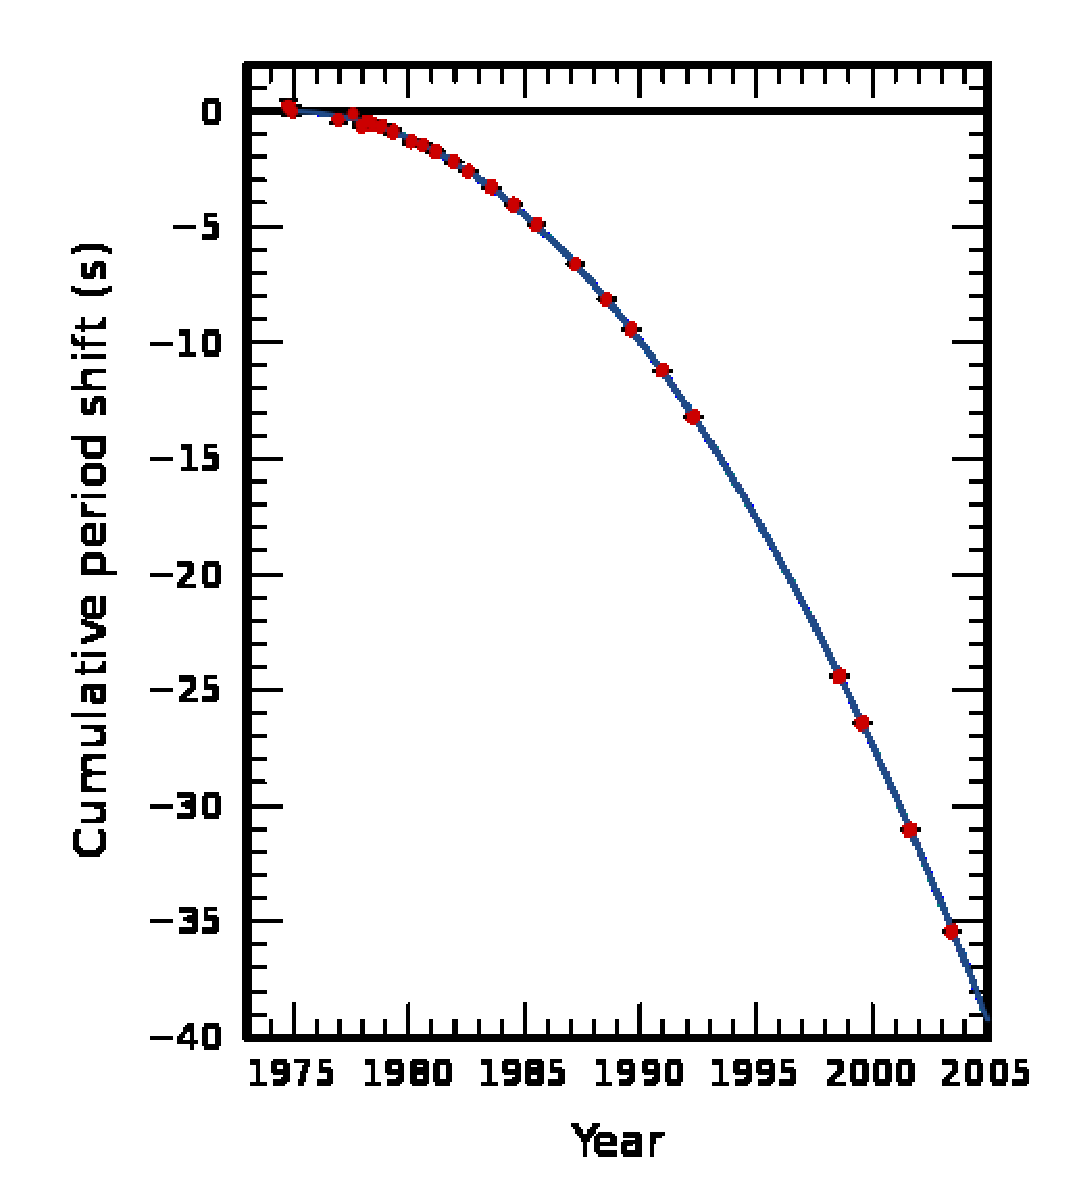
\includegraphics[height=111mm, width=148mm]{500px-PSR_B1913+16_period_shift_graph.eps}
	\caption{The Hulse-Taylor binary PSR 1913+16, orbital period change over time consistent with emission of gravitational radiation from its system~\cite{Weisberg2010}. Gravitational waves emission depletes orbital energy, causing the binary stars to slowly inspiral into closer orbits. Shrinking pulsar radius $R$ leads to the shorter period $T$ -- Kepler's third law, $T \propto R^{3/2}$ (first stated in \textit{Harmonices Mundi}~\cite{Hawking2002}). Timing error can be ruled out, because the orbital decay is not linear.}
	\label{Hulse-Taylor_binary}
	\end{center}
	\end{figure}

Before delving into general relativitic emission, let us consider the astrophysical sources expected to emit gravitational waves. 
Physics prompts our search, but astronomy makes it exciting.
When gravitational waves are heard by the interferometers, the public should remember them as the songs of dead stars, rippling through the fabric of spacetime.  
Gravitational waves (henceforth also abbreviated GW) searches presently focus on four distinct types of cosmic sources.
This categorization of sources was presented no later than the 1983 LIGO Blue Book proposal and has since guided research focus~\cite{CollinsGravityShadow,Schutz1989}. 
The quadripartite division:
\begin{itemize}
\item Burst (rarely, `supernova')
\item Compact binary coalescence (or `inspiral')
\item Continuous wave (or `pulsar')
\item Stochastic
\end{itemize}

This thesis concentrates on continuous waves -- sine waves. 
Continuous waves (CW) are most likely to emanate from neutron stars. 
Perhaps neutron star CW modulated by orbital motion, spun-up from accretion or spun-down from radiated energy. 
Given a sufficiently large ellipticity, on the order of $\epsilon \approx 10^{-7}$~\cite{Owen2005} or smaller for a neutron star rotating on the order of 1 kHz, a deformation of the crust would radiate sufficient gravitational radiation to be a plausibly-detectable source. 
Indeed, the radiation would rapidly deplete the rotational energy of the neutron star~\cite{Owen1998}, which is why binary systems, where the neutron star could be recycled and spun-up by a partner, prove a promising target~\cite{PapaloizouPringle1978,Wagoner1984}. 
Scorpius X-1 offers a canonical case~\cite{AbbottScoX12007}, although the TwoSpect search anticipates an abundance of other low-mass X-ray binary (LMXB) systems of interest. 
Given the paucity of insight on the interiors of collapsed stellar remnants, direct detection of GW from neutron stars would prove informative. 
Just as we might infer details from neutron star binary coalescences favoring one equation of state~\cite{Lattimer2007,Read2009}, we might also extract parameters from continuous waves suggesting the existence of quark stars or gravitars~\cite{Owen2005}, and will have an unparalleled peek into the interior of the densest stable three-dimensional objects in the universe. 
Their simple waveforms might even facilitate the calibration of other types of GW data, whereas binary mergers should sound like standard sirens to compare against electromagnetic and neutrino observations~\cite{Punturo2010}
(see next paragraph).
CW are conceptually-elegant and astronomically-enticing.
Yet other sources of GW, have a comparable pull on our attention. 

Inspirals or compact binary coalescences occur when two stellar remnants draw nearer in their orbits, radiating gravitational radiation and finally merging in a titanic release of energy. 
While sometimes invisible -- the merging of black holes in short-hard gamma ray burts (GRBs) being an exception -- these events compete eagerly with supernovae as the most explosive in the modern universe. 
Were GW observatories to see their waveforms, they could be compared with those predicted through post-Newtonian approximation and numerical relativity. 
As GW amplitude should diminish linearly with distance, we would then have standard candles or \textit{standard sirens} by which to calibrate and measure the universe. 
Advanced LIGO may prove sensitive to neutron star-neutron star and stellar mass black hole-neutron star mergers, and, if low-frequency sensitivity is sufficient and the sources exist, to intermediate-mass black holes. 
Space-based observatories such as the longsuffering Laser Interferometer Space Antenna (LISA) and ensuing DeciHertz Gravitational-wave Observatory (DECIGO) \& Big Bang Observer (BBO) could detect supermassive black hole mergers. If launched, they would see a low-frequency noise floor due not to seismic vibration, as in LIGO, but to white dwarf binaries throughout the galaxy. 
Since the waveforms are well-predicted, we could even investigate deviations from general relativity, perhaps seeing new physics in the ringdown of black holes.

Physical insight could also come from burst searches. 
Bursts share with inspiral searches the property of looking for a single event, as opposed to a source spread over long duration. 
Analytical programs for bursts can sometimes be applied to inspiral or detector characterization tasks as well; rare noise events are a limit on their astronomical sensitivity.
Yet the immediate focus lies with supernovae and perhaps gamma-ray bursts. 
Because the waveform is unknown, burst searches rely significantly more on the coincidence between multiple detectors to distinguish signal from noise. 
Just as with neutrino observations of supernova 1987A, the burst program would hope for a fortuitously nearby cataclysm to be seen simultaneously -- or nearly so, the time of flight indicating a direction -- in a global gravitational-wave detector network. 
Due to the versatility of this method, some researchers have proposed looking for longitudinal polarization in addition to plus and cross orthogonal polarization (possible in non-general relativistic terms; see Section~\ref{history_GR}). 
Any detection would be quiet exciting for probing systems still mysterious with electromagnetic and neutrino measurements, and it would help, in conjunction with multi-messenger coordinated searches with those observatories, to ascertain at precisely what speed gravity travels through space-time and to what extent it is attenuated or altered.

The background of space-time itself may hide GW signatures. 
Searches for the stochastic GW background look not for single events but for persistent phenomena buried in many months of correlated signals between networks of detectors. 
In doing so, they hope in particular to see the earliest turbulence of the universe -- long before the cosmic electromagnetic background, now microwaves, was emitted 380000 years after the Big Bang, GW were travelling unimpeded. 
While the opacity of the infant cosmos conflates electromagnetic signals from different times and places, the transparency of the universe to gravity means that we might see the inflationary epoch or earlier, the Planck time. 
Unfortunately, this signal is thought to be far below the sensitivity of existing detectors. 
While LIGO did set a new upper limit on the energy density of GW, measured as a fraction, $\Omega_{gw}$ of the critical closure density of the universe~\cite{LIGOStochasticNature2009}, the inflationary background at LIGO frequencies is predicted to be about ten orders of magnitude lower. 
Alternative theories, such as ekpyrotic/cyclic universes, make other predictions, so an anomalously high stochastic background could prove cosmologically significant.

All GW searches would open up new directions in astronomy. 
While the most exciting possibility is that we will see the unexpected, we think that our present algorithms will permit serendipity while efficiently categorizing computational challenges. 
Continuous wave and inspiral methods both search against waveform templates; burst and stochastic have no template and rely on correlation and coincidence. 
Continuous wave and stochastic analyze weeks, months, even years of data in search of persistant features; inspiral and burst look for transient events. 
In the abstract dimensions of search groups, we are complete. 
Our blind spots are in what data we provide to those groups -- in the focus on audio frequencies of tens to a few thousand Hertz at present -- blindness that will in time be rectified by CMB polarization, pulsar-timing and space-based interferometry for low frequencies and possibly by atom interferometry for high frequencies. 
To appreciate our choice of focus in these nascent days of the field, we must turn back a century to understand its origins in Einstein's mathematics.

        \subsection{History from general relativity}
        \label{history_GR}

            %Historical brief of Einstein.
        Einstein's theory unified a sequence of historical insights. 
Since 1676, when Roemer used the moons of Jupiter to measure the finite speed of light, just before Newton's 1687 \textit{Principia Mathematica}~\cite{Hawking2002}, the question of gravity's propogation beckoned. 
Bringing together the work of Minkowski and Poincar\'{e}, the 1905 special theory of relativity highlighted the naturalness of the speed of light, but only in 1915, with the presentation of the Einstein field equations of general relativity, based in Riemannian geometry, did a means to an answer emerge. 
In 1916, Einstein predicted GW. 
At last, gravity had a theoretical speed: the same as that of electromagnetism, that of light in the vacuum, $c$.
In the linear approximation to the nonlinear theory of general relativity (henceforth GR), the waves were mathematically similar to the waves of electromagnetism, as will be shown in Section~\ref{general_relativity}.
GR offers a consistent explanation for how changes in the distribution of matter change gravitational fields.
Yet the detectability of the waves, even in principle, would remain an open question for another half century. 
Uncertainty in whether fluctuations within spacetime could be detectable with instruments themselves changed by the fluctuations dominated the debate.
Consult Misner, Thorne, and Wheeler's \textit{Gravitation}~\cite{MisnerThorneWheeler} and Sean Carroll's lectures notes~\cite{Carroll1997}, as well as other history books of the field for an account of the controversy.
Thought notions, \textit{Gedankenexperiment}, such as beads-on-rods led to consensus that GW carried and could deposit physical energy and thus be detected. 
See \textit{Gravity's Shadow}~\cite{CollinsGravityShadow} for sociological perspective, and 
\textit{Gravity's Ghost}~\cite{CollinsGravityGhost} for insight into the detection criteria that have since evolved\footnote{See also a recent review by Riles~\cite{Riles2013}.}.

Discussions of GW frequently begin with derivations of the wave equations from Einstein's field equations. 
General relativity, however, is not the only theory to predict GW: waves are a natural consequence of a class of similar theories, which make a range of testable predictions (such as number of polarization modes, from two to six, and possibly speeds different from $c$)~\cite{Will1993} 
Waves should thus be expected even if some minor variation from Einstein's theory is discovered, pointing a way perhaps toward a quantum theory of gravity~\cite{Sathyaprakash2009}. 
%As the field progresses toward first detection and beyond to astronomy, the astrophysical targets of our searches should take precedence.

Before deriving the answer to the detectability question from the field equations, a contrast with the situation in other fields of astronomy is in order.

 
        \subsection{Contrast with electromagnetic and particle astronomy}
        \label{contrast_astro}

        With astronomy, detection came first, then theory.
Visible light astronomy began with the earliest humans.
Records of the star Sirius are known from Egyptian astronomers, the planet Venus from Babylonians, sunspots from the Chinese, and eclipses from the Greeks. 
Thus the telescope, though revolutionary, was not unimaginable.

Infrared radiation, as first seen by William Herschel, was just beyond the visible red light of a prism.
As the wave nature of light came to be understood, culminating in Maxwell's equations, the existence of invisible electromagnetic radiation was put on sound theoretical footing.
The only remaining questions pertained to whether this radiation would prove astornomically interesting, especially in the extreme low- (radio) and high- (X- and $\gamma$-ray) frequencies found at the end of the 19th Century.
Fortuitiously, unlike with GW today, these novel bands of electromagnetic spectrum could be easily generated and detected by scientists in small laboratories, as with Marconi and Marie \& Pierre Curie.
Within half a century, radio telescopy began with Karl Jansky.
By the early 21st Century, radio astronomy ranged from common rooftop designs~\cite{SRT} (nonetheless sensitive enough to infer the galactic rotation curve in the hydrogen line~\cite{MeadorsThesis2008}) to planetary-scale very long baseline interferometry and plans for a Square Kilometer Array.
Electromagnetic, or photon, astronomy has the advantage of calibration with familiar sources.

%            Contrast with electromagnetism, compare with radio/X-ray/et cetera astro. 

%Can make analogy to radio waves and make note of the ease with which one can operate a small radio telescope, as I did in my thesis~\cite{MeadorsThesis2008}, compared the the difficulty of GW detection. 

Other particles besides the photon began to play a role in 20th Century astronomy.
Muons from space were detected long ago, as in C.D. Anderson's 1949 paper on what was then called the mesotron~\cite{CDAnderson}. 
Solar neutrinos were, after much difficulty, seen by John Bahcall~\cite{NeutrinoReview}, and neutrino astronomy is a well-established field by the turn of the millenium, following the detection of Supernova 1987A in the Large Magellenic Cloud. 
New types of neutrino detectors (for example, time-projection chambers~\cite{EBubble2005,MeadorsNevis2006}) could yield additional information and better sensitivity, but as with electromagnetism, the calibration question is resolved. 
Since the Savannah River nuclear reactor experiments, the experimental detectability of neutrinos has been settled, and though the 1964 theory of solar neutrinos~\cite{NeutrinosSolarTheoretical} required tuning to account for neutrino oscillation, astrophysics with neutrino observatories is becoming mature.
Nuclear fusion in the Sun has been well-established, and arrays such as Antares and IceCube will move the field outwards toward cosmic sources.


 GW from the PSR 1913+16 pulsar itself~\cite{WeisbergTaylor2004} are too low in frequency to be seen with existing interferometers, but they confirm that the phenomena is real.
Although no terrestrial sources of GW can be feasibly generated, calibration~\cite{AbadieCalibration2010} of interferometers is nonetheless accurate to a few percent.
Direct detection of GW would let us infer the true strength of astrophysical gravitational radiation and compare that power with theory. 
Surprising new insights are probable in any new field, not unlike the discovery of neutrino oscillation in the solar spectrum or the anomalous galactic rotation curve due to dark matter, are probable in any new field.

Yet how can gravity been seen?
GW are conceptually simple, with mathematics illustrated by electrodynamic analogy in the Appendix.
A short derivation follows.

    %End section by very rapidly deriving wave equation of electricity and magnetism, to lead by example for how we go about GR.
    %Note that all physics in min(action),
    %introduce metric as inner product
    %generally, coordinate transform good



    \section{General relativity}
    \label{general_relativity}

        Einstein's theory of General Relativity (hence GR) describes gravitation as a pseudoforce. 
Unlike Newton, Einstein posits that objects always follow an extremized path, $\delta s = 0$ for arclength $s$  -- a geodesic worldline -- when the curvature of spacetime is considered. 
This supposition follows from the Fermat principle of least time.
In turn, Fermat inspired the least action principle, $\delta S = 0$.
Likewise, the following discussion of GW interferometry is best understood in terms of phase or \textit{time-of-flight}.
The curvature of spacetime is described by the Riemann tensor, $R^\mu_{\nu\rho\sigma}$, which is a solution to the Einstein field equations. 
In Section~\ref{field_equations} the connection between these field equations and the Ricci scalar curvature will be clarified. 
This Riemann tensor can be constructed from the Christoffel connection, $\Gamma^\mu_{\rho\sigma}$, which in turn can be expressed in terms of the metric, $g_{\mu \nu}$.
Whereas electromagnetism arises from $U(1)$ unitary Lie group gauge symmetries, general relativity arises from $GL(4, \mathbb{R})$ general linear Lie group symmetries.

 Carroll and \textit{Gravitation} are essential references~\cite{Carroll1997,MisnerThorneWheeler}, consulting other sources for the Einstein-Hilbert/Palatini action~\cite{FarrThesis}.

%            Introduce the metric $g$ here, but reinforce that it is not essential.
%Intro to GR -- right motivation is least action Ricci tensor, implying field equation and phase/time-of-flight implying interferometry.

        \subsection{Symmetry and action principles}
        \label{principles}

            Like electricity and magnetism, GR is the product of symmetry, action. 


        \subsection{Derivation of field equations}
        \label{field_equations}

            A common approach to GW derivations is linearized GR~\cite{FlanaganHughes2005}.
            This approach is correct in weak fields, and proceeds~\cite{AdhikariThesis} from the metric $g$ approximation as the sum of a Minkowski (flat spacetime) component, $\eta$, plus a perturbation $h$, where $|h| \ll |\eta|$:

\begin{equation}
g_{\mu \nu} \approx \eta_{\mu \nu} + h_{\mu \nu},
\end{equation}

\noindent leading to a wave equation,

\begin{equation}
-\frac{1}{2} \Box \left(h_{\mu \nu} - \frac{1}{2} \eta_{\mu \nu} h_{\lambda}^{\lambda} \right) = \frac{8 \pi G}{c^4} T_{\mu \nu}.
\end{equation}

The wave carries energy~\cite{BallmerThesis} as well:

\begin{eqnarray}
\rho_{\textup{gw}} = \frac{c^2}{16 \pi G} \left\langle |\partial_t h_+|^2 + |\partial_t h_\times|^2 \right\rangle,\\
P = \frac{G}{5c^5}\left\langle \left( \partial_t^3 I_{ij}\right)^2  \right\rangle \approx 5.5\times 10^{-54} W^{-1} \left\langle \left( \partial_t^3 I_{ij}\right)^2  \right\rangle.
\end{eqnarray}

Let us demonstrate this result and also derive field equations from the action, integrating over extremized curvature~\cite{FarrThesis}.
Obtain the action from Ricci scalar curvature $R$, a hypothetical constant, $\Lambda$ (termed the cosmological constant), and the matter Lagrangian density $\mathcal{L}_M$:

\begin{equation}
\mathcal{S} = \int \left( R - 2\Lambda + \mathcal{L}_M \right) \sqrt{-|g|}d^4 x,
\end{equation}

Given $R = R^\mu_\mu$ Ricci scalar a for a $R_{\mu\nu} = R^\lambda_{\mu\lambda\nu}$ Ricci tensor contracted from the Riemann tensor, $R^\mu_{\nu\rho\sigma}$ (the curvature tensor, equivalently the 2-form $\textsf{R}^\mu_\nu$), we can construct the Maurer-Cartan structure equation with a connection $\omega$,

\begin{eqnarray}
\textsf{R}^\mu_\nu = d\omega^\mu_\nu + \omega^\mu_\rho \wedge \omega^\rho_\nu, \\
\omega^{\rho'}_{\mu\sigma'} = e^{\alpha'}_{\nu} e^{\lambda}_{\beta'} \Gamma^{\nu}_{\mu\lambda} - e^{\lambda}_{\beta'} \partial_{\mu} e^{\alpha'}_{\lambda},\\
\Gamma^\sigma_{\mu\nu} = \frac{1}{2} g^{\sigma\rho} \left( g_{\nu \rho, \mu} + g_{\rho \mu, \nu} - g_{\mu\nu,\rho} \right). 
\end{eqnarray}

\noindent where the last equation defines the \textit{Christoffel} connection. Then we obtain the \textit{Einstein field equations}, sourced by the stress-energy tensor, $T_{\mu\nu}$:

\begin{equation}
R_{\mu} - \frac{1}{2} R g_{\mu\nu} + \Lambda g_{\mu\nu} = 8 \pi T_{\mu\nu}.
\end{equation}

\noindent These are nonlinear, but when linearized, there is indeed a wave solution: $\Box h_{\mu\nu} = 0$~\cite{Carroll1997}
The wave, parametrized by path $x^\mu (\lambda)$ follows the usual geodesic equation, where the covariant derivative by $\mu$ of $V^\nu$ is defined by $\nabla_\mu V^\nu = (\partial_\mu V^\nu + \Gamma^\nu_{\mu\lambda} V^\nu)$ and along a path by $D_\lambda = dx^\mu_\lambda \nabla_\mu$,

\begin{equation}
D_\lambda \partial_\lambda x^\mu = 0
\end{equation}

The wave has plus $h_+$ and cross $h_\times$ polarizations, making the metric waveform along the $z$-axis ($k_\mu = \textup{diag}(\omega,0,0,1)$) in transverse-traceless gauge:

\begin{equation}
h_{\mu\nu} =
\left[
\begin{array}{cccc}
0 & 0 & 0 & 0\\
0 & -h_+ & h_\times & 0 \\
0 & h_\times & h_+ & 0\\
0 & 0 & 0 & 0
\end{array} \right] \cos \left(k_\mu x^\mu \right).
\end{equation}



        \subsection{Radiation from quadrupoles}
        \label{radiation}
  
            Predict power from rotating quadrupole. Might also be a good place to invoke Vladimir's thesis~\cite{DergachevThesis} as well as original primary sources. Note that just as light travels at the speed of light, which is measureable~\cite{CODATA} and which can be derived from electromagnetic theory~\cite{GriffithsE}, so we think that gravity should travel at the speed of light. Note that this radiation should not be affected by the interstellar medium. I think that Ostriker is the source to reference on the ISM~\cite{Caldwell1981},~\cite{McKee1977}.

    \section{Astrophysical estimates}
    \label{estimates}

        Astrophysical estimates and predictions.

        \subsection{Sources: burst, continuous, inspiral and stochastic}
        \label{source_types}

            %Describe the four types of sources: burst, continuous, inspiral and stochastic.

            Let us summarize, more briefly, the current state of the art in each search, describing the four types of searches: burst, continuous, inspiral, and stochastic, with reference to a review by Riles~\cite{Riles2013}.

		Mostly above, but clarify exact how much we should see. Cite the 2009 Nature stochastic paper et al~\cite{LIGOStochasticNature2009}. The importance to early universe cosmology was initially handled by Maggiore~\cite{Maggiore2000}. Before that, of course, once can reference the Allen and Romano methods paper~\cite{Allen1999}, anything interesting from Nick Fotopoulos's thesis~\cite{FotopoulosThesis}, and the various mid-2000s stochastic work that I was familiar with~\cite{Abbott2006},~\cite{Abbott2007}. Note the interesting meaning of anisotropies~\cite{Allen1997} and point out how not only Stefan's radiometer search can find them but how it can be adapted to many other purposes, such as spherical harmonics, which is useful for the cosmic microwave background~\cite{Muciaccia1997} and was briefly my work~\cite{MeadorsCaltech2007} and the Scorpius X-1 search; Stefan's canonical radiometer reference is in Classical Quantum Gravity~\cite{Radiometer2006}.

        \subsection{Continuous waves from neutron stars}
        \label{continuous_waves}

            Continuous -- specifically, binary neutron stars and rate predictions. Describe archetypical search methods as in the 1998 analysis paper~\cite{Jaranowski1998}, the Abbott et al paper~\cite{LSCPulsar2006}, including StackSlide~\cite{LSCPulsarS4}, Einstein at Home~\cite{LSCEinsteinHome2009}, and the most interesting to date from Michigan, Vladimir's PowerFlux~\cite{LSCPowerFlux2009}. Discuss earlier results from the earliest period~\cite{Abbott2004} and an early search for Scorpius X-1~\cite{AbbottPulsar2006}. Reinhard Prix is probably another good source~\cite{Prix2006}.
Promising searches have been carried out by the LIGO Scientific Collaboration for the Crab and Vela pulsar remnants.

		Rates go in here.
        The emission mechanism of gravitational radiation with amplitude $h_0$ from a neutron star is is from an elliptical deformation, ellipticity $\epsilon$, on its surface, leading to a quadrupole moment $I$~\cite{Zimmermann1979,LSCPulsar2006} and thus emission at frequency $f = 2\nu$, twice the neutron star spin frequency $\nu$:

        \begin{eqnarray}
        \epsilon = \frac{I_{xx} - I_{yy}}{I_zz}, \\
        h_0 = \frac{4 \pi^2 G}{c^4} \frac{I_{zz} f^2}{r} \epsilon.
        \end{eqnarray}

Excepting the case of torque balance in low-mass X-ray binary systems, neutron star rotation frequency will decay due to gravitational radiation, yielding a relationship between the `spindown age'~\cite{Brady1998} $\tau$ and the gravitational radiation amplitude:

        \begin{eqnarray}
        \tau = -f / \dot{f}, \\
        h_0 = \frac{1}{r} \sqrt{\frac{5 G I_{zz}}{2 c^2 \tau}}.
        \end{eqnarray}

	\begin{figure}
	\begin{center}
	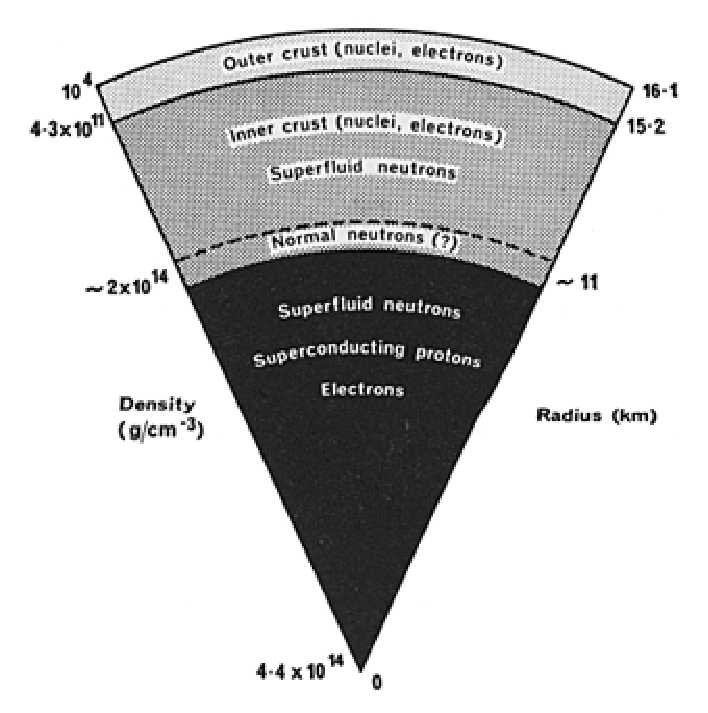
\includegraphics[height=111mm, width=148mm]{neutron_star_structure.eps}
	\caption{Hypothetical internal structure of a neutron star (Citation: \url{http://heasarc.gsfc.nasa.gov/docs/objects/binaries/neutron_star_structure.html})} 
        %CITE Possibly original Frank Shu? Fred would probably know, being a student of Frank
	\label{neutron_star_structure}
	\end{center}
	\end{figure}


    \section{Laser Interferometer Gravitational-wave Observatories}
    \label{LIGO}
        
        LIGO observatories. The most fun part to write. Cite Nergis Mavalvala~\cite{MavalvalaThesis}, Stefan Ballmer~\cite{BallmerThesis}, Rana Adhikari~\cite{AdhikariThesis}, Nicolas de Mateo Smith-Lefevbre~\cite{SmithThesis} and, of course, Peter Saulson~\cite{Saulson}.

        \subsection{From Weber bars to interferometry}
        \label{bars_to_interferometry}

            History lesson: Weber bars progress to interferometers. Use Saulson, but Nic's thesis has links to some of the original sources~\cite{Saulson},~\cite{SmithThesis}.           

        \subsection{Observatories, investigations, and enhancements}
        \label{methods}

		Michelson was one of the first to use interferometers~\cite{michelson}. He is famous for having done so to try to measure the velocity of the Earth with respect to the luminerferous ether and finding it to be unmeasurable.

A GW interferometer, at its core, is also a Michelson interferometer. 
The power $P$ at the output `dark' port, is by design equal to zero except when the measureable (e.g., ether, a GW, or other disturbance) causes a fringe shift $\Delta \phi$ related to the agnular frequency $\omega$ of the light and the time-of-flight down the $x$ and $y$ arms, $T_x$ and $T_y$. 
Physically, it is proportional to the electric field: 

\begin{eqnarray}
P \propto E_0^2 \left| 1 + e^{i \Delta \phi}\right|^2 = 2 E_0^2 (1 + \cos \Delta \phi), \\
\Delta \phi = \omega (T_y - T_x).
\end{eqnarray}

In Enhanced and Advanced LIGO, $\Delta \phi = 2\pi L_s /\lambda + \phi_0 + \phi_{\textup{DARM}} $, where in decreasing order of size, $L_s$ is known as the Schnupp asymmetry (a constant difference in arm length), $\phi_0$ is a constant offset from a fringe to enable non-radio-frequency-modulated DC readout, and $\phi_{\textup{DARM}}$ is the putative time-varying signal of `DARM', the differential arm motion that might encode a GW signal. 

Power $P$ can be directly improved by increasing effective laser power (e.g., a brighter laser or use of `power recycling'), and $\delta \phi$ can be increased by making $T_{x,y}$ storage times longer (e.g., with Fabry-Perot cavities).

Gravitational wave signals enter the interferometer, in a technical sense, by changing the spacetime curvature in the arms. It is not necessary to discuss mirror motion or Doppler shifting, although these are also valid points of view. 

In the simplest, linearized picture, the spacetime curvature leads to a GW with amplitude $h$; when the wave is aligned with x-axis and y-axis arms of length $L$ (see~\cite{Jaranowski1998} for the antenna pattern correction when it is misaligned), it changes the time-of-flight in the arms:

\begin{eqnarray}
T_x = \int_0^{\frac{2L_x}{c}} \sqrt{|g_{xx}|} dt \propto \int_0^{\frac{2L_x}{c}} \left(1 - \frac{h_+}{2} \right) dt, \\
T_y = \int_0^{\frac{2L_y}{c}} \sqrt{|g_{yy}|} dt \propto \int_0^{\frac{2L_y}{c}} \left(1 + \frac{h_+}{2} \right) dt.
\end{eqnarray}

\noindent The mismatch in the integrals leads to a detectable time-varying signal,

\begin{equation}
\phi_{\textup{DARM}} = \omega \int_0^{\frac{2L}{c}} \frac{h_+ (t, x(t)) + h_+ (t, y(t))}{2} dt.
\end{equation}  



            Why GW interferometers work. Null measurements, a zeroed operating point. The specifics are best handled by Saulson~\cite{Saulson}. The idea of a Pound-Drever-Hall lock is most elegantly explained by Black~\cite{PDHNotes}. Rai Weiss may have some neat details, possibly historical, albeit that it is in a presentation~\cite{LIGOWorks}. The details of Fabry-Perot cavities in LIGO are handled by Rakhmanov, Savage et al~\cite{ResonanceFP},~\cite{ResponsesFP}. The motivation for the evolution to Enhanced LIGO and its DC readout methods is covered well in the corresponding CQG article~\cite{Fricke2009} and specific details of its construction and operation are in Tobin Fricke's thesis~\cite{FrickeThesis}.

            \subsubsection{Interferometer theory}
            \label{interferometer_theory}
        
                GW interferometry theory: differential arm motion, key noise sources. Again, the main source is Saulson~\cite{Saulson}, although we also need another source in the Advanced Detector Era.

                Here we discuss the key noises sources: seismic noise, thermal noise, and quantum (radiation pressure, shot noise).

                Arms are locked using the Pound-Drever-Hall technique, as elucidated in Section~\ref{phase_camera}, which discusses how the electro-optic modulations (EOMs) provide an error signal for locking the Fabry-Perot arms.
See Figure~\ref{primary_eLIGO_optics}

\begin{figure}
\begin{center}
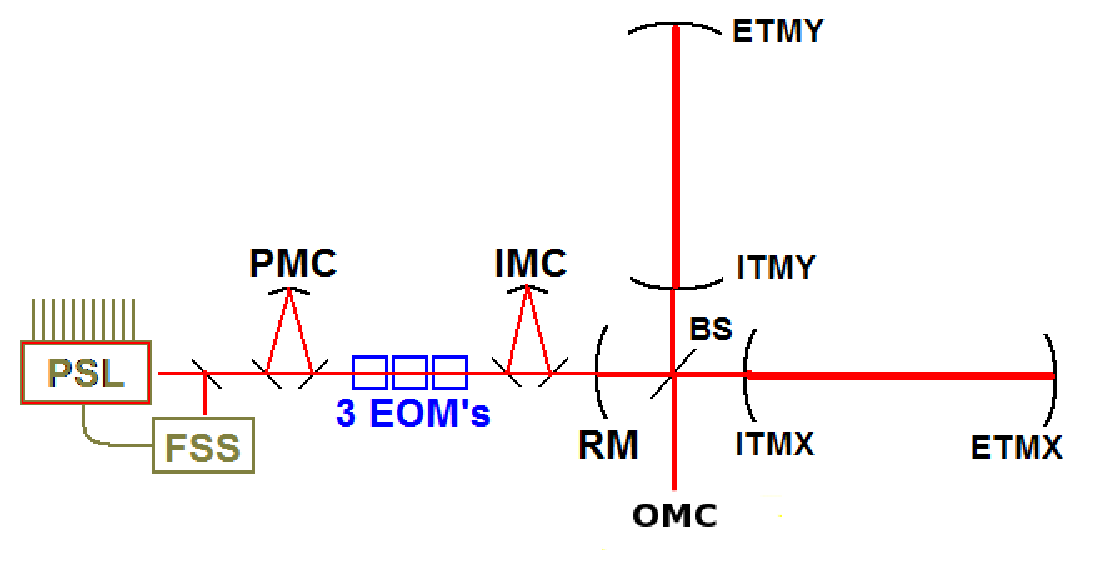
\includegraphics[height=111mm,width=148mm]{LIGODiagramnew.eps}
\caption{Enhanced LIGO primary systems and optics. From left, the phase-stablized laser (PSL) produces coherent light, kept at constant frequency by the frequency-stabilization servo (FSS). The pre-mode cleaner excludes non-Gaussian beamshapes, allowing only the $TEM_{00}$ mode to pass. The beam is the phase-modulated using three electro-optical modulators (EOMs) before being further shaped in the input mode cleaner (IMC). The beam passes through the power recycling mirror (RM) and is split at the beam-splitter (BS). Along the $X$ and $Y$ arms, light resonates in the Fabry-Perot cavity formed between the input test mass (ITM) mirror and the end test (mass) ETM mirror, before recombining at the beamsplitting. Any light with the same phase as before the arms is returned to the interferometer by the RM, but if phase-shifted, perhaps by a gravitational wave, it exits through the output mode cleaner (OMC): a photodiode just downstream of the OMC records the signal.}
\label{primary_eLIGO_optics}
\end{center}
\end{figure}

            \subsubsection{Observatory operation}
            \label{observatory_operation}

                Operating LIGO: controls, Detector Characterization. One of the first sources from initial LIGO to read up on is a paper by Fritscel, Bork, Mavalvala et al~\cite{ReadoutGWA}. Initially this system made a detection based on heterodyne readout using GW sidebands, which, among other troubles, could be unequal in the recycling cavity~\cite{MeadorsHanford2005}.

	\begin{figure}
	\begin{center}
	\includegraphics[height=111mm, width=148mm]{Screen_shot_2010-07-21_at_042516.eps}
	\caption{Screenshot of MEDM control panel. MEDM is a Motif Epic and Display Manager for EPICS, the Experimental Physics and Industrial Control System, which lets operators control LIGO. MEDM allows operators to run locking scripts as well as alignments and tests, and to activate and de-activate filters.}
	\label{ScreenshotMEDM}
	\end{center}
	\end{figure}

Features of initial and enhanced LIGO:
\begin{itemize}
\item Power recycled Michelson interferometer with Fabry-Perot arms
\item Hanford, Washington and Livington, Lousiana observatories
\item 4 km perpendicular beam tubes
\item $10^{−9}$ torr vacuum
\item 20 W Nd:YAG 1064 nm laser
\item 10 kg fused silica primary optics
\item 4-stage seismic isolation
\item Laser frequency stabilization
\item Angular sensing and control (wavefront sensors, optical levers)
\item Length sensing and control (magnet coils, common mode)
\item Pre, input, and output mode cleaning
\item Power recycling
\item Digitally filtered servos and readout
\end{itemize}


                \paragraph{Detector characterization}
                \label{detchar}
            
                    DetChar methods: omega scans, line hunting and glitches

My work on site included getting the Omega scan engine tested and running manual Omega scans in the first months of S6, July and August 2009. 
See Figure~\ref{omega_scan_audible_glitch} for an example of the spectrograms this method was able to generate. These spectrograms helped categorize glitch sources and reduce them, to the benefit of the burst group in particular.
Fortunately, this work was later automated thanks to Tomoki Isogai. 


\begin{figure}
\begin{center}
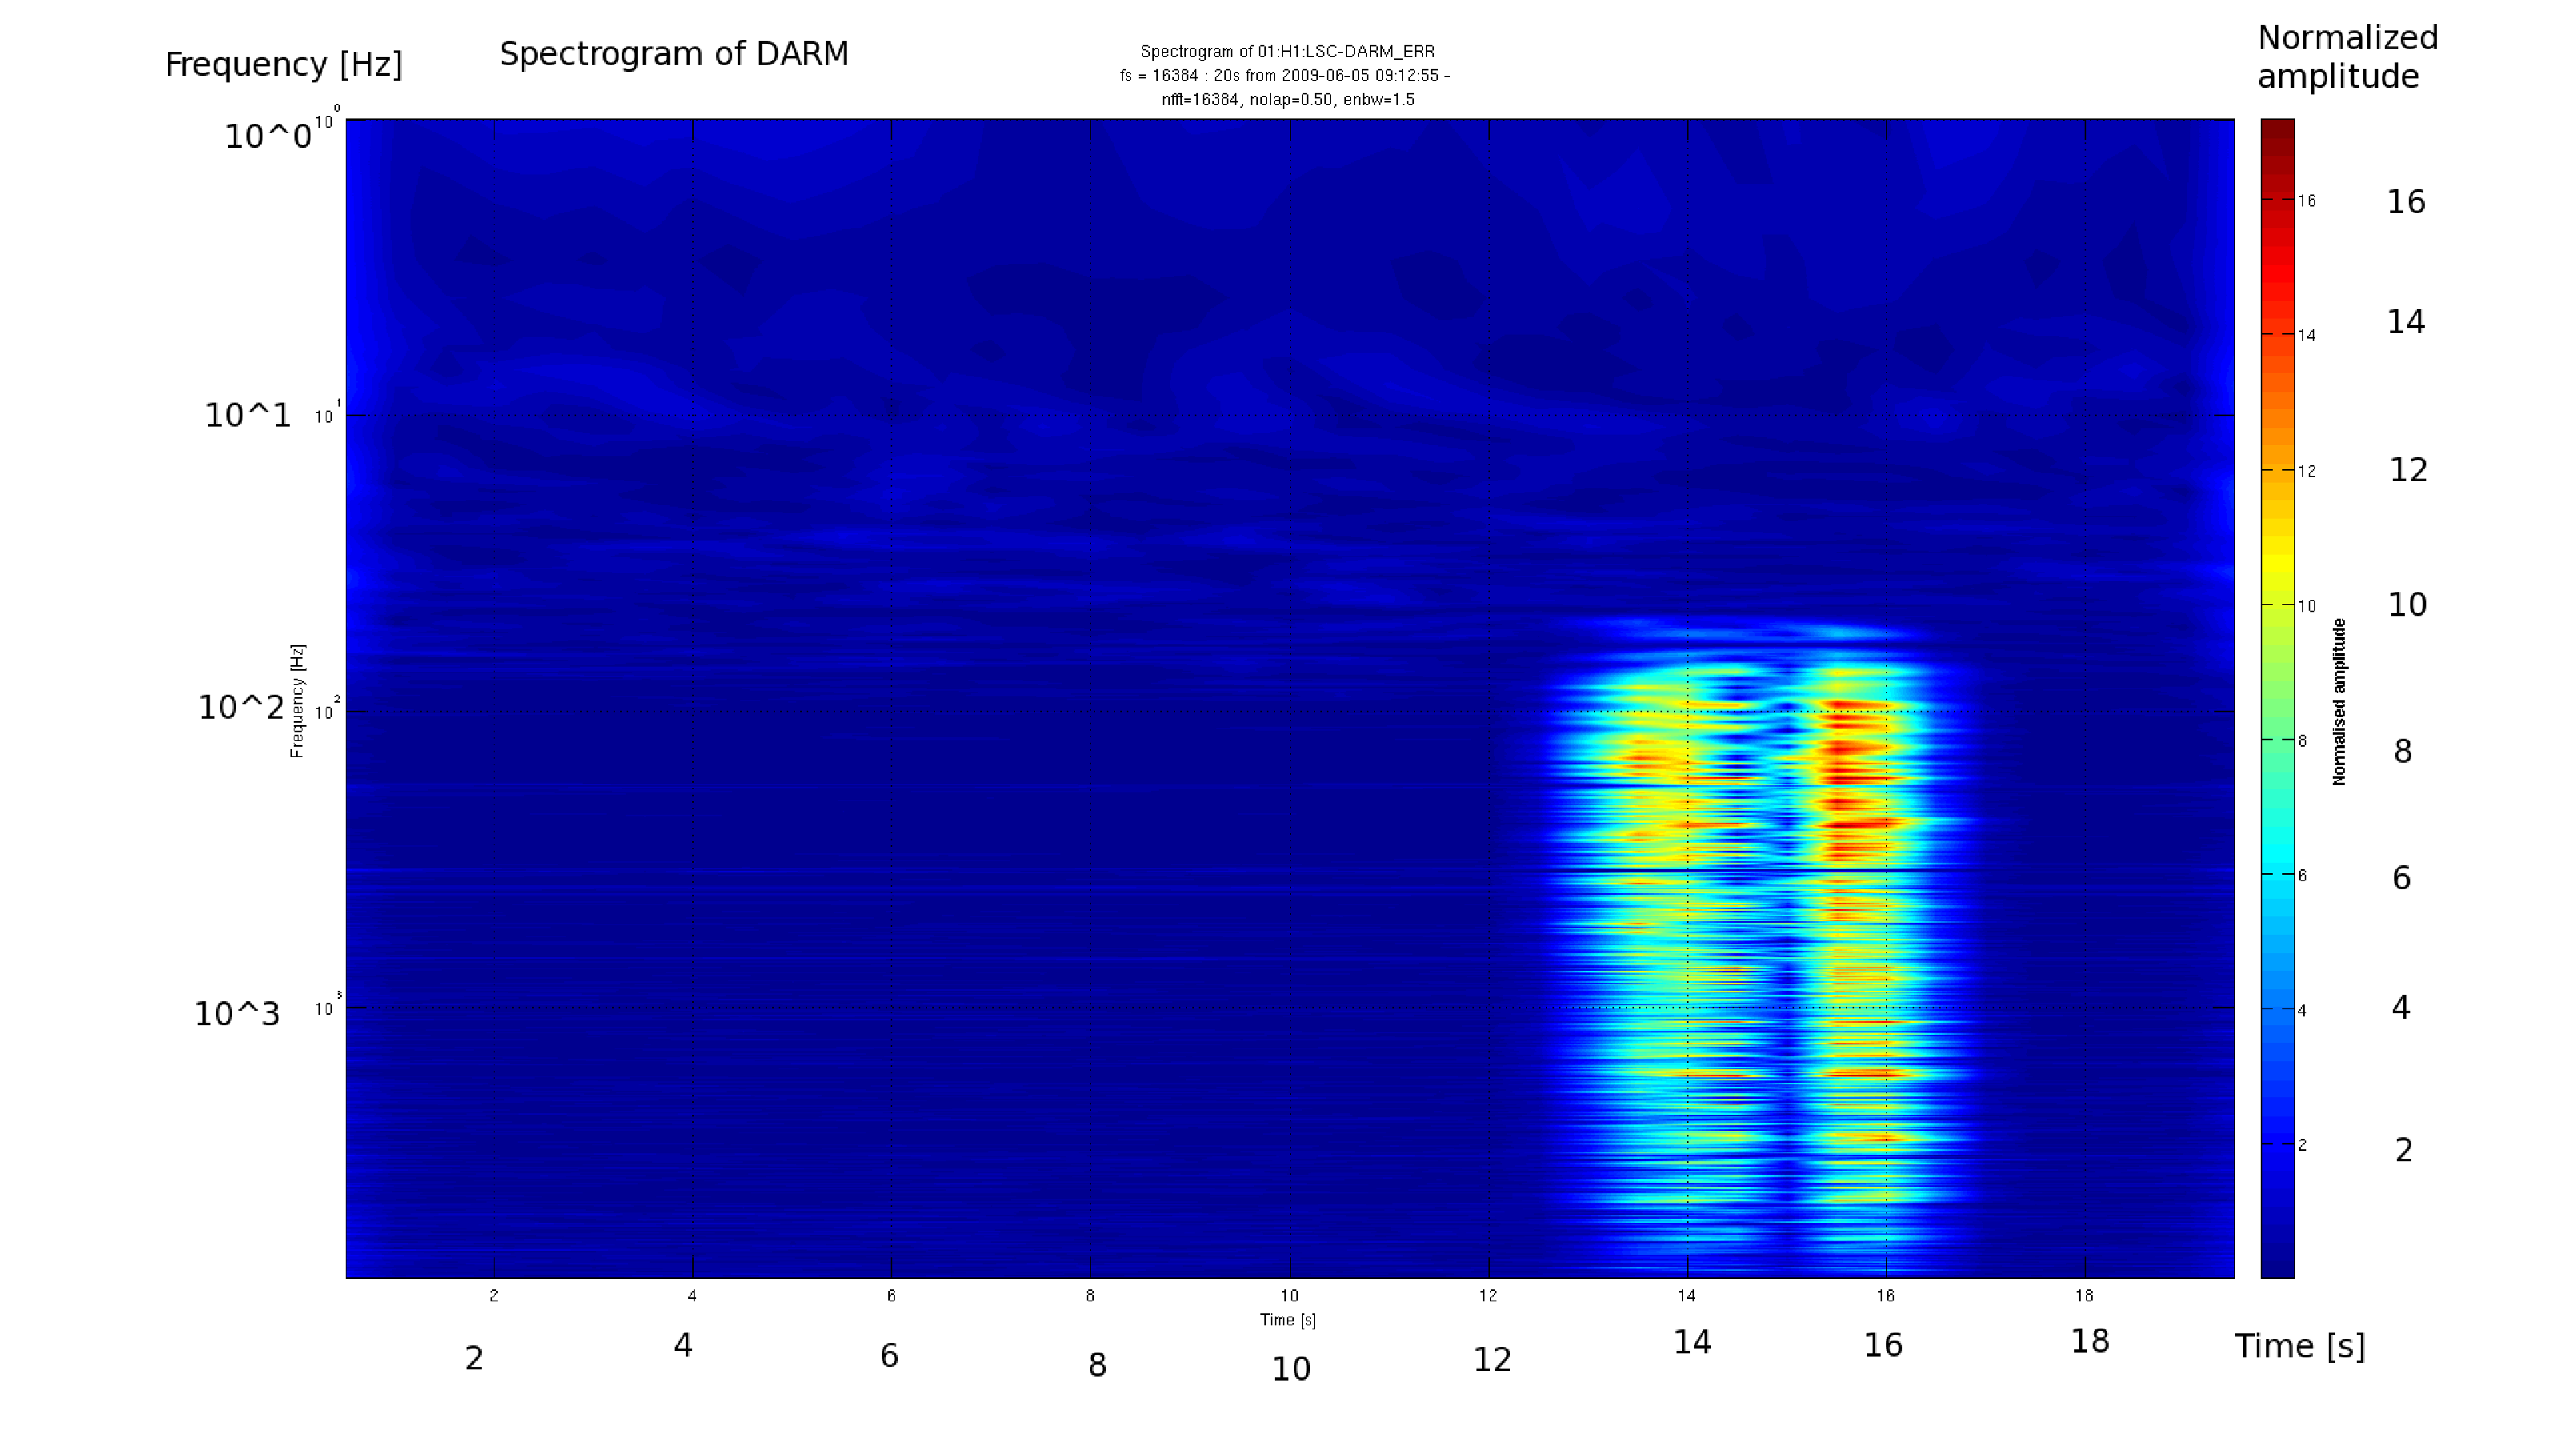
\includegraphics[height=111mm, width=148mm]{aglitch928228390_new.eps} 
\caption{Omega scan of an audible broadband glitch. Shortly before the start of Science Run 6, detector characterization took place to identify categories of glitches, such as the `gremlin', and to eliminate them. The burst group analysis pipeline, Omega, generated time-frequency spectrograms that made this identification easier. Glitches are a limiting factor in the identification of rare events and therefore of potential gravitational wave burst signals.}
\label{omega_scan_audible_glitch}
\end{center}
\end{figure}

                \paragraph{Feedforward filtering}
                \label{feedforward_filters}

                    Example of feedforward: 60 Hz magnetometer. The only source that mentions this is, I think, Nic's thesis~\cite{SmithThesis}. Yet the most pertinent example is one that has long been applied to LIGO: MICH and PRC feedforward. The specific needed are mention in the thesis of Adhikari~\cite{AdhikariThesis} and Ballmer~\cite{BallmerThesis}, but immediately before Keita Kawabe and I began our project, these parameters had been tuned by Jeff Kissel~\cite{KissellPRCMICH}

	\begin{figure}
	\begin{center}
	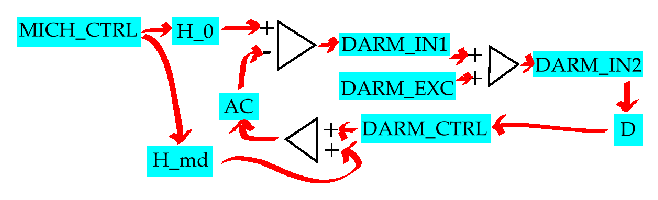
\includegraphics[height=80mm, width=148mm]{servo_loop.eps}
	\caption{Real-time servo loop diagram. The MICH\_CTRL signal can be though to leak into the true DARM signal via a transfer function, H\_0. (The letter `h' is typical for transfer functions as well as gravitational wave strain; coincidentally, this is a noise transfer into the channel for displacement, DARM, which is proportional to strain $h(t)$). H\_0 leaks into error signal, which is otherwise kept null thanks to the servo cancellation provided by DARM\_CTRL times a physical actuation function AC. The measured error signal is DARM\_IN1. If desired, an excitation can be supplied via DARM\_EXC for a sum of DARM\_IN2. This error signal passes though digital filters D to yield the aforementioned control signal DARM\_CTRL. The auxiliary length cancellation loop is simply adding H\_md to DARM\_CTRL in order to subtract out the corruption of H\_0.}
	\label{servo_loop_realtime}
	\end{center}
	\end{figure}

	\begin{figure}
	\begin{center}
	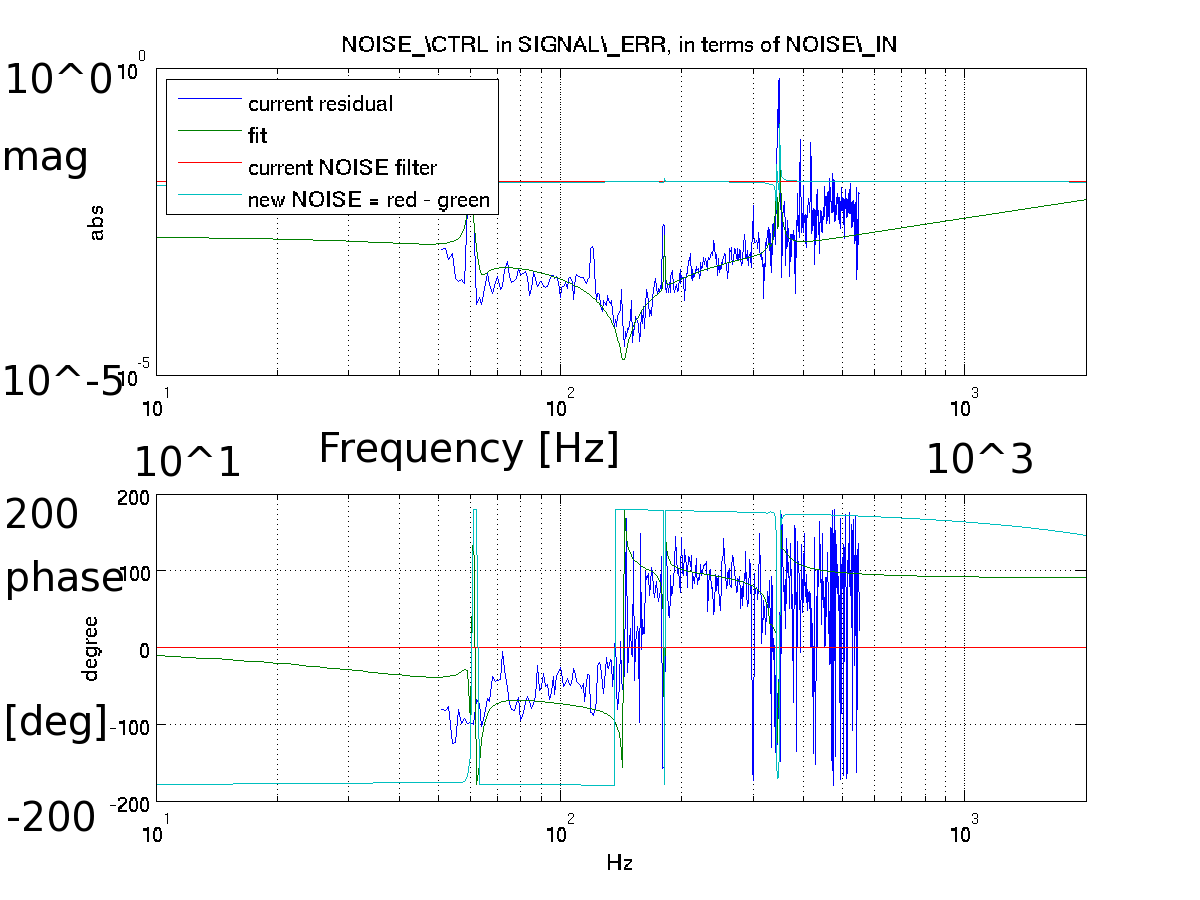
\includegraphics[height=111mm, width=148mm]{newNOISEfilter.eps}
	\caption{Real-time work on a LIGO noise filter. This Bode plot, made in Matlab, shows the correction to the existing MICH damping (cancellation) loop needed mid-2010, toward the end of Science Run 6. The correction is small, because the majority of the coupling fits the flat model expected from theory. This transfer function estimate suffices for post-factor correction. However, in order to be incorporated into the control scheme shown in Figure~\ref{servo_loop_realtime}, measurements of the open loop gain $G$ and actuation function AC are necessary to yield incorporate the filter correctly into the closed loop response.} 
	\label{newNOISEfilter}
	\end{center}
	\end{figure}

The closed loop gain mentioned in Figure~\ref{newNOISEfilter} is a function of frequency because it is a geometric sum of time $\tau$-delayed open loop gain responses by DARM\_CTRL to error signals from DARM\_ERR: $G_\textup{closed} = \lim_{p\rightarrow\infty} \Sigma_n^p G e^{i n \omega \tau} = \left(1 + G e^{i \omega \tau} \right)^{-1}$. 
Because MICH damping is summed with DARM\_CTRL, it picks up an additional factor of the actuation function AC for a net transfer function of $H_{md} G_\textup{closed}$AC in the closed loop. 
Thus, compared to an open-loop (e.g., post facto) subtraction, a real-time servo will differ by a factor of $G_\textup{closed}$AC. 

	\begin{figure}
	\begin{center}
	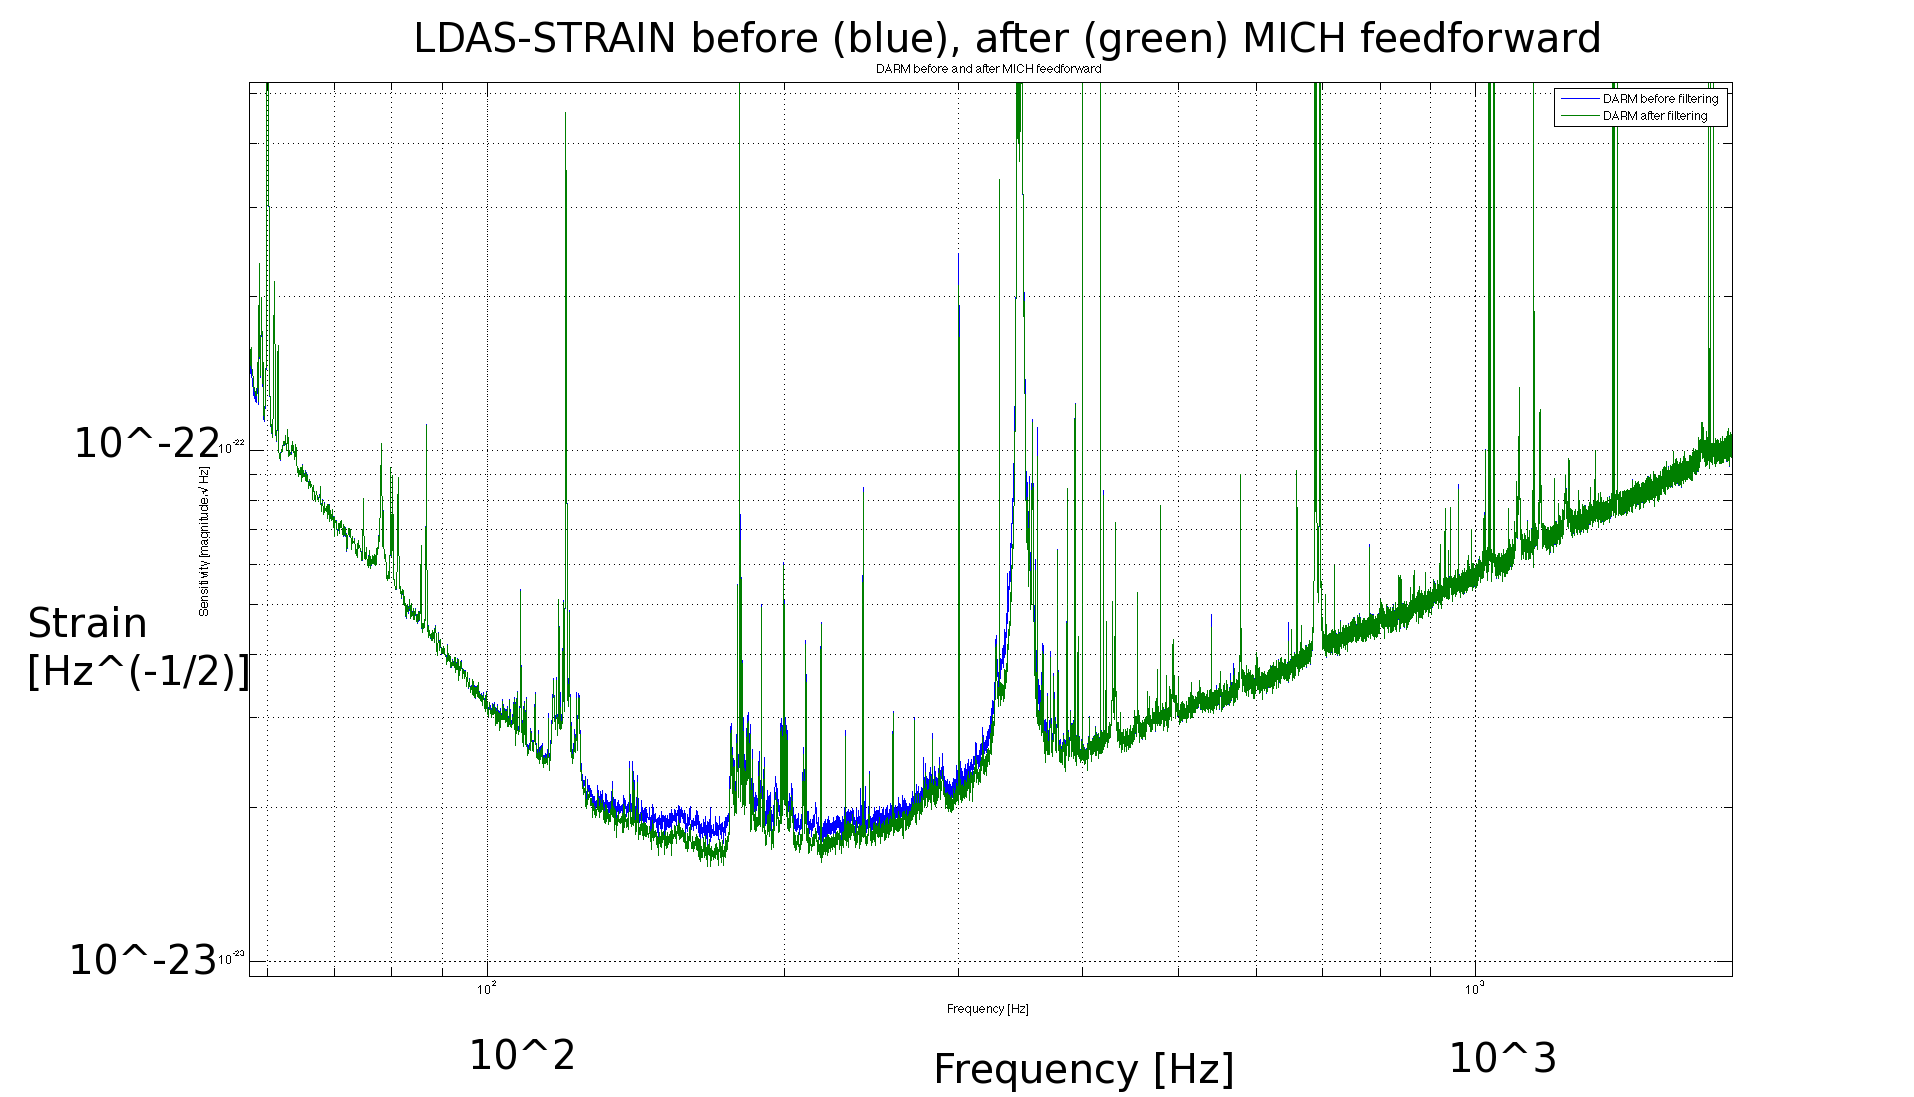
\includegraphics[height=111mm, width=148mm]{2011-03-08_filter-01.eps}
	\caption{Early work on post-facto noise filtering. After testing out MICH damping filters offline, post-facto, the correction factors for AC and $G_\textup{closed}$ were incorporated and the entire filter imported using Foton into the EPICS control system, where it was used real-time from the September equinox of 2010 until the end of Science Run 6.}
	\label{filter_early}
	\end{center}
	\end{figure}

                \paragraph{Phase camera}
                \label{phase_camera}

                    Future devices: overview of phase camera with Vladimir. Vladimir's thesis definitely talks about it~\cite{DergachevThesis}. We can discuss the fundamentals behind the need for angular stabilization and control from Nergis Mavalvala's thesis~\cite{MavalvalaThesis}, but we can refresh it with a modern reference from Kate Dooley's thesis~\cite{DooleyThesis}.

The electronics development were guided by Horowitz and Hill~\cite{HorowitzHill1989} as well as by Simpson~\cite{Simpson}.

Locking used the Pound-Drever-Hall (PDH) method~\cite{PDHNotes,MavalvalaThesis}.
Mathematically, the method assumes two mirrors: an input, with amplitude reflectivity $r_1$, and an end, with amplitude reflectivity $r_2$.
Upon the input mirror is incident a coherent electric field, due to light, $E_\textup{inc}$ at frequency $\omega_0$. A field $E_{\textup{refl}}$ is reflected.
The key to the technique is that the incident electric field is phase modulated by a factor $\Gamma$ with modulation frequency $\Omega$, by a device such as an electro-optic modulator (EOM, e.g., a Pockels cell).
Typically this modulation is done at radio-frequency.
This EOM modulates an electric field of amplitude $E_0$ into higher and lower frequency sidebands, amplitude $E_+$ and $E_-$, as determined by expansion in Bessel functions $J_n(\Gamma)$ -- higher order sidebands exist at usually-negligible amplitude.
From the reflected signal, then, the intensity $I$ encodes an error signal of the arm length $l$, for given light wavenumber $k = \omega / c$, at the modulation frequency (aside from additional signals at DC and at 2$f$):

\begin{eqnarray}
E_{\textup{refl}} = \frac{r_1 - r_2 e^{-2 i k l}}{1 - r_1 r_2 e^{-2 i k l}} E_\textup{inc},\\
E_\textup{inc} = E_0 e^{i \Gamma \cos \left( \Omega t \right)} \approx E_0 e^{i \omega_0 t} \left[ J_0 (\Gamma) + J_1 (\Gamma) e^{i\Omega t} + J_{-1} (\Gamma) e^{-i \Omega t} \right],\\
E_\textup{refl} \approx e^{i \omega_0 t} \left[ E_0^\textup{refl} + E_+^\textup{refl} e^{i\Omega t} + E_-^\textup{refl} e^{-i \Omega t}\right],
\end{eqnarray}
\begin{equation}
\begin{split}
I =& \left[ |E_0|^2 + |E_+|^2 + |E_-|^2\right] + \\ 
  & \left[(E_0^* E_+ + E_0 E^+_-)e^{i\Omega t} +\textup{C.C.} \right] + \\
  &\left[E_+ E_-^* e^{2i\Omega t} +\textup{C.C.} \right].
\end{split}
\end{equation}

Radio-frequency photodiode can record this intensity.
Typically, the photodiode current is demodulated with a mixer that uses as local oscillator the same sine wave that drives the Pockels cell EOM phase modulation.
See Figure~\ref{phase_camera_optical_table} for a picture of the cavity as built.

\begin{figure}
\begin{center}
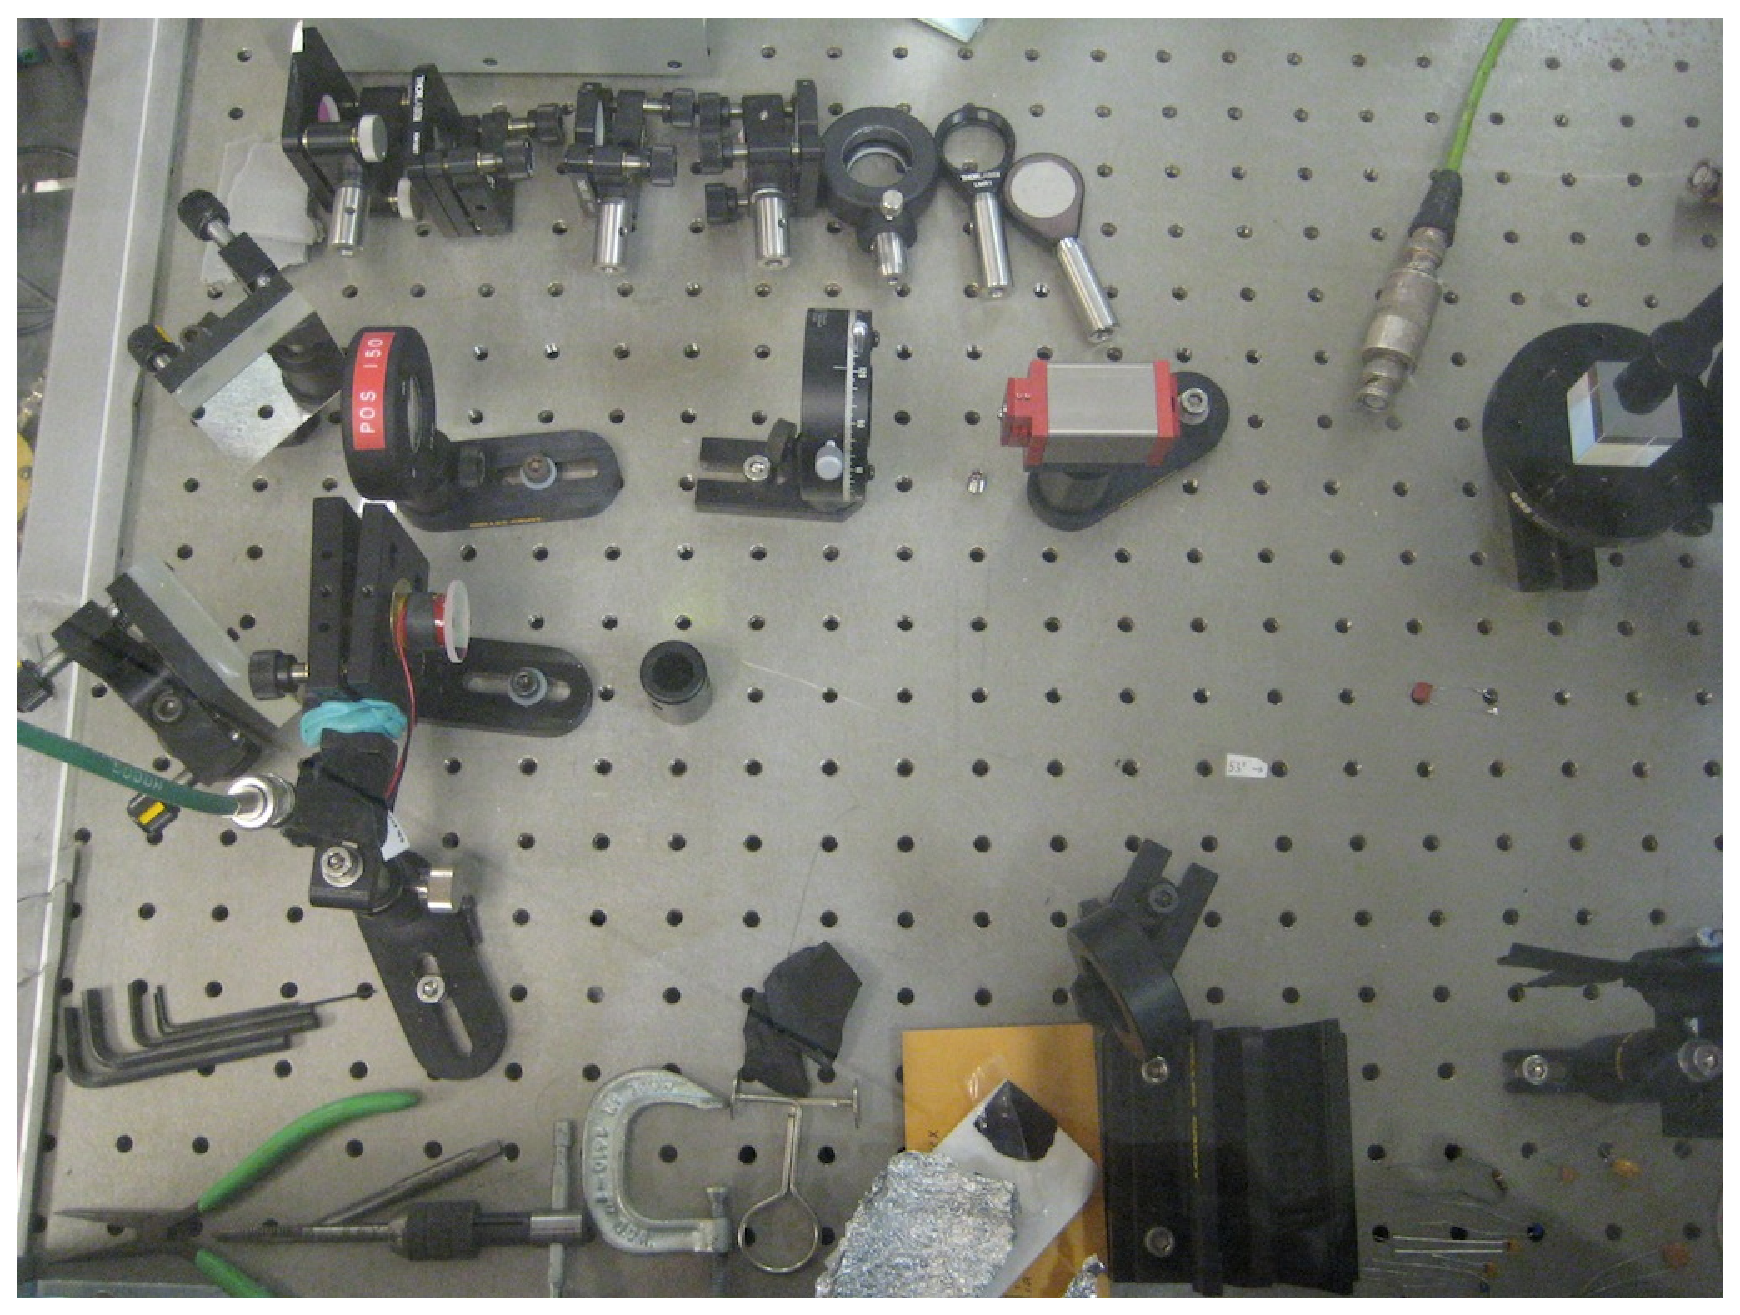
\includegraphics[height=111mm, width=148mm]{Optical_table_phase_camera.eps}
\caption{Optical table layout with Fabry-Perot cavity and Pound-Drever-Hall locking for phase camera. Faraday isolator and polarizing beam-splitter at upper right; piezoelectrically-actuated mirror at center left. Difficulties with stability, despite a plexiglass enclosure and floated table, meant that locks were fractions of a second at most, hampering efforts.}
\label{phase_camera_optical_table}
\end{center}
\end{figure}

        \subsection{Advanced observatories and beyond}
        \label{advanced}
  
            Advanced LIGO and beyond -- squeezing and prospects?

        \subsection{Worldwide network}
        \label{worldwide}
 
            Allies: LIGO India, KAGRA, Advanced VIRGO, Einstein Telescope, LISA

    \section{Summary}
    \label{intro_summary}
 
        %Summary: strong motivation and instruments, need to find evidence of GW.    

Initial LIGO, during the science runs S6, would have been able to see the coalescence of two neutrons stars at about twenty Megaparsecs, out in the Virgo cluster of galaxies, from sixty-five million years ago, when dinosaurs still walked the Earth. 
In the first week of Advanced LIGO lock at Livingston, following Memorial Day 2014, Advanced LIGO had a temporal range extending only as far back as when early humans began their diaspora from Africa -- a terrestrial parallel to the expansion of the cosmos.
When completed, the Hanford and Livingston second-generation interferometers should see back ten times beyond what S6 could, six hundred and fiften million years, to before the Cambrian explosion of life.
Perhaps in the third or fourth generation of interferometers, our view of the gravitational sky may stretch back the age of the observable universe.
Even then, we will not have seen all that can be seen.
With the two long-range forces of the universe, electromagnetism and gravitational, giving two complimentary views of spacetime, we still must build great machines to explore the sights they show, we must understand what we are seeing, and we must propogate that understanding. 

This thesis is a prelude to those efforts, from the building of the quantum optical squeezer, and the feedforward regression and continuous waves binary search, to our public interferometer exhibitions.   
Feedforward regression provides a microcosm of the complexities of gravitational wave interferometry, so there we will begin.


            
%        --------------------
%
%	Here is a sample chapter file. The chapters of the thesis
%	should be saved to seperate files such as
%	\textit{chapter1.tex}. In the file \textit{thesis.tex} the
%	\textit{input} command then includes these chapters into the
%	thesis. Note that none of the chapter files need any headers.
%	This header for each of these files is contained in
%	\textit{thesis.tex}. The file \textit{thesis.tex} also
%	includes the numbers system for the sections, figures,
%	theorems lemmas etc...

%\section{Sample Section}
%\label{sample_section}
%
%	This is what a sample section looks like. Let's conclude this
%	section with a sample theorem statement and proof.
%
%	\begin{theorem}
%	\label{sample_theorem}
%	The are an infinite number of prime numbers
%	\end{theorem}
%
%	\emph{Proof:} On the contrary assume there are a finite number
%	of primes $P_1, P_2, ... P_n$. Consider $\mathcal{P} = P_1 P_2
%	\cdots P_n+1$. $\mathcal{P}$ is not divisible by any of the
%	primes in our finite set. (Contradiction) $\square$
  

